% This is LLNCS.DEM the demonstration file of
% the LaTeX macro package from Springer-Verlag
% for Lecture Notes in Computer Science,
% version 2.4 for LaTeX2e as of 16. April 2010
%
\documentclass{llncs}
%
\usepackage{makeidx}  % allows for indexgeneration
\usepackage{graphicx}
%
\begin{document}
%

%
\title{Documentatie MySSH}
%
\author{Covaliu Lucian}

\institute{Facultatea de Informatica Iasi}

\maketitle              % typeset the title of the contribution

%
\section{Introducere}
%
Proiectul MySSH utilizeaza arhitectura client-server pentru a asigura o executie sigura printr-un canal criptat a comenzilor date de client pe server.
%
\section{Tehnologii utilizate}
%
%
\subsection{Thread-uri}
%
Serverul MySSH va fi unul multithreaded pentru a permite executia comenzilor de la mai multi utilizatori in acelasi timp.Solutia aleasa prezinta avantajul folosirii a mai putine resurse decat in cazul unui server multiproces. De asemenea abordarea multi-threaded asigura o performanta sporita, in special pe sistemele multiprocesor, unde thread-urile pot rula separat pe unitati centrale de procesare diferite.Comunicarea intre thread-uri este de asemenea mai facile decat comunicarea intre procese.
%
\subsection{TCP}
%
Aplicatia va folosi protocolul TCP deoarece conexiunile sunt doar point-to-point si asigura transmiterea in siguranta si in ordine a datelor, un aspect vital al aplicatiei. De asemenea conexiunea se stabileste o singura data, la deschiderea aplicatiei iar toate tranzactiile de tip cerere-raspuns sunt transmise prin aceasta, deci desi conexiunea se stabileste mai incet decat in cazul UDP aceasta se realizeaza o singura data, impactul asupra performantei fiind mai scazut decat in cazul trimiterii prin UDP.
%
\subsection{Criptare}
%
Pentru a asigura un canal de comunicare sigur aplicatia va folosi medote moderne de criptare atat pentru credentialele utilizatorului folosing un algoritm de hashing cat si pentru transmiterea tranzactiilor cerere-raspuns printr-un algoritm care foloseste o cheie publica de criptare.
%
\subsection{SQLite}
%
Stocarea credentialelor fiecarui utilizator se va face folosind o baza de date SQLite. Baza de date poate fi accesata de mai multe thread-uri in mod concurent si mai multe cereri de citire pot fi satisfacute in paralel astfel oricati utilizatori se pot loga in acelasi timp
%
\section{Arhitectura aplicatiei}
%
\begin{figure}
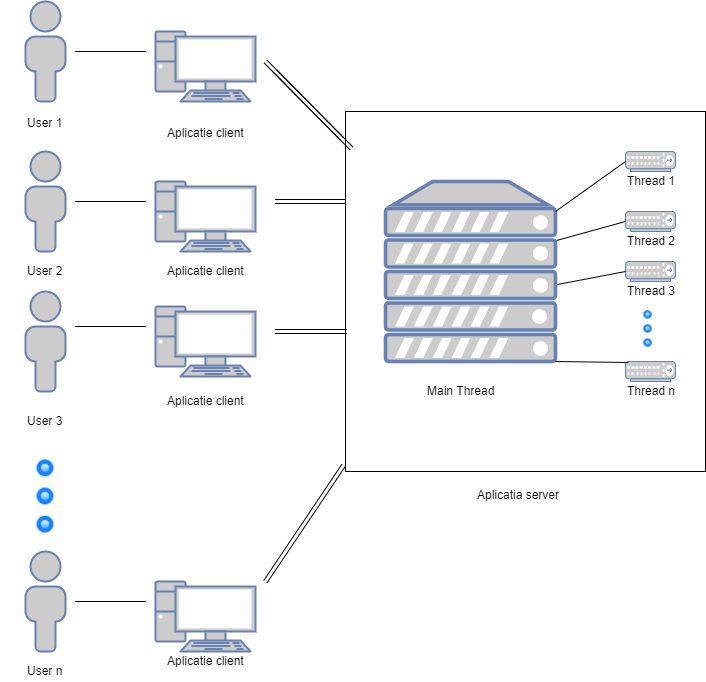
\includegraphics[width=\linewidth]{diagram.png}
\end{figure}
Fiecare utilizator se va conecta la server prin intermediul aplicatiei client. Pe server, thread-ul principal va astepta conexiuni, iar la cerea de conexiune a unui client va crea un nou thread care va stabili o conexiune cu clientul. Fiecare thread va avea acces la baza de date astfel se va putea efectual login-ul apoi transmiterea tranzactiilor cerere-raspuns.
%
\pagebreak
\section{Detalii de implementare}
%
\begin{figure}
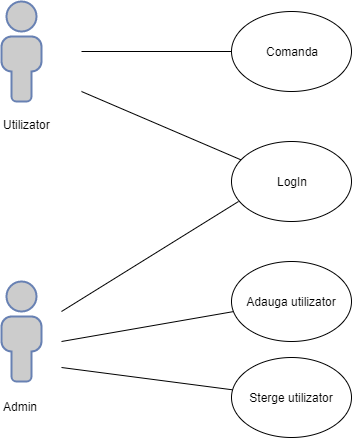
\includegraphics[width=0.5\linewidth]{Usecase.png}
\end{figure}

In momentul conectarii la server, utilizatorului ii este cerut numele si parola, fara un cont utilizatorul nu poate continua. Datele contului sunt stocate pe server intr-o baza de date SQLite, parola fiind hash-uita folosing un algoritm de criptare. Dupa ce utilizatorul a trimis un nume si o parola valida acesta poate executa comenzi pe server. Canalul de comunicare va fi de asemenea criptat folosing un algoritm cu cheie publica de criptare.\\

Exista un cont unic de administrator care poate adauga sau sterge utilizatori dupa ce acesta s-a logat.

\subsection{Cereri}
\begin{figure}
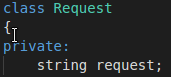
\includegraphics[width=0.4\linewidth]{request.png}
\end{figure}

O cerere la server contine un string cu comanda pe care utilizatorul doreste sa o execute. Inainte de trimiterea acesteia se trimite un integer care reprezinta marimea cererii.
%

\subsection{Raspunsuri}
\begin{figure}
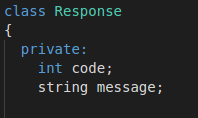
\includegraphics[width=0.4\linewidth]{response.png}
\end{figure}

Raspunsurile de la server sunt de asemenea precedate de marimea acestora. Acestea contin un mesaj: output-ul comenzii rulate sau mesajul de eroare si un cod, acesta specifica in ce fel s-a executat comanda si care este eroarea in cazul in care exista una.\\

Codurile sunt numere de trei cifre, codul pentru succes este 100, codurile pentru erori la client incep cu 2, codurile pentru erori la server incep cu 3 iar codurile pentru erori la executia comenzii incep cu 4. Celelalte doua cifre vor preciza care este eroarea pentru a fi afisat un mesaj corespunzator pentru utilizator in cazul in care campul cu mesaj nu contine unul.\\

Exemplu de eroare la citirea marimi raspunsului de la server:

\begin{figure}
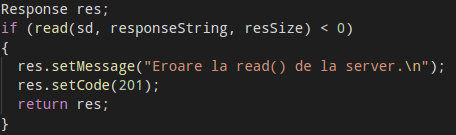
\includegraphics[width=\linewidth]{exerr.png}
\end{figure}

%
\section{Concluzii}
Datorita unor situatii neprevazute cererile si raspunsurile se pot modifica pe parcursul dezvoltarii aplicatiei, dar ideea de baza ramane aceeasi.\\
%

\begin{thebibliography}{}
%
\bibitem{2clar:eke}
Cursurile de retele de calculatoare: \\https://profs.info.uaic.ro/~computernetworks/cursullaboratorul.php
\bibitem{2clar:eke}
Lista de proiecte: \\https://profs.info.uaic.ro/~computernetworks/ProiecteNet2017.php
\end{thebibliography}

\end{document}
